%!TEX root = ./template-skripsi.tex
%-------------------------------------------------------------------------------
%                            BAB II
%               KAJIAN TEORI
%-------------------------------------------------------------------------------

\chapter{KAJIAN TEORI}                

\section{\textit{Tracer Study} (Studi Penelusuran)}

Menurut Nuryake Fajaryati et al dalam Jurnal ELINVO Vol 1 No 1 (2015), \textit{tracer study} merupakan studi yang tujuan utamanya untuk memperoleh informasi mengenai lulusan yang sudah bekerja dan belum bekerja. Selain itu \textit{tracer study} bertujuan untuk mengetahui hasil pendidikan dalam bentuk penguasaan dan pemerolehan kompetensi lulusan yang diaplikasikan di dunia kerja serta transisi dari dunia pendidikan tinggi ke dunia usaha dan industri. Melalui \textit{tracer study} ini penyelenggara pendidikan dapat mengetahui bagaimana penyelenggaraan dan mutu layanan program melalui penilaian para alumni sehingga mampu untuk memperbaiki dan meningkatkan kualitas layanannya \cite{Nuryake}. 

\textit{Tracer study} adalah studi penelusuran jejak lulusan dilakukan setelah kelulusan dan bertujuan untuk mengetahui \textit{outome} pendidikan dalam bentuk transisi dari dunia pendidikan tinggi ke dunia kerja. Memberikan informasi mengenai \textit{output} pendidikan yaitu penilaian diri terhadap penguasaan dan pemerolehan kompetensi, proses pendidikan berupa evaluasi proses pembelajaran dan kontribusi pendidikan tinggi terhadap pemerolehan kompetensi serta input pendidikan dalam bentuk penggalian lebih lanjut terhadap informasi sosiobiografis lulusan \cite{ExploringTS}.

Berdasarkan uraian di atas \textit{tracer study} adalah suatu studi yang dilakukan untuk menggali informasi terkait kondisi alumni, yaitu dalam masa transisi dari pendidikan tinggi ke dunia kerja, bertujuan untuk mengetahui hasil dari proses pendidikan suatu perguruan tinggi berupa kompetensi lulusan, hasil yang didapat dijadikan bahan evaluasi bagi perguruan tinggi untuk meningkatkan mutu layanan atau program pendidikannya. Menurut Soemantri (2010) dalam \textit{Jurnal Electronics, Informatics, and Vocational Education (ELINVO)}, Volume 1, Nomor 1, November 2015, terdapat tiga manfaat yang dapat diperoleh dari pelaksanaan t\textit{racer study}, yaitu \cite{Nuryake} :
\begin{enumerate}
	\item Mengetahui kepuasan \textit{stakeholders}, dalam hal ini lulusan, terkait dengan \textit{learning experiences} yang mereka alami, untuk dijadikan alat evaluasi kerja institusi.
	\item Mendapatkan masukan yang relevan sebagai dasar pijakan pengembangan institusi, terkait dengan kemampuan bersaing, kualitas, dan \textit{working experiences} lulusan yang bisa digunakan untuk menangkap kesempatan dan menanggulangi ancaman ke depan. 
	\item Meningkatkan hubungan lulusan dan almamater, karena apabila dilihat dari pengalaman institusi-institusi pendidikan terkenal, ikatan lulusan dan almamater yang kuat akan membawa banyak manfaat kepada almamater seiring dengan diakuinya kiprah lulusan di masyarakat. 
\end{enumerate}
	
\section{Sistem Informasi}
Sistem Informasi terdiri dari kata sistem dan informasi. Sistem adalah kumpulan orang yang saling bekerja sama dengan ketentuan-ketentuan aturan yang sistematis dan terstruktur untuk membentuk satu kesatuan yang melaksanakan suatu fungsi untuk mencapai tujuan. Sedangkan informasi adalah data yang diolah menjadi lebih berguna dan berarti bagi penerimanya, serta untuk mengurangi ketidakpastian dalam proses pengambilan keputusan mengenai suatu keadaan. Sistem informasi merupakan suatu kombinasi teratur dari orang-orang, \textit{hardware}, \textit{software}, jaringan komunikasi dan sumber daya data yang mengumpulkan, mengubah, dan menyebarkan informasi dalam sebuah organisasi \cite{Elisabet}

Menurut Sebastian K Boell dan Dubravka Cecez-Kecmanovic (2015), Sistem Informasi melibatkan berbagai teknologi informasi seperti komputer, perangkat lunak, basis data, sistem komunikasi, internet, perangkat seluler dan masih banyak lagi, untuk melakukan tugas tertentu, berinteraksi dengan dan memberi tau berbagai pengguna dari organisasi yang berbeda \cite{Sebastian}. Sistem Informasi dari suatu organisasi terdiri komponen-komponen berikut \cite{Muslihudin} :

\begin{enumerate}
	\item Perangkat keras, yaitu perangkat keras komponen untuk melengkapi kegiatan memasukkan data, memproses data, dan keluaran data.
	\item Perangkat lunak, yaitu program dan instruksi yang diberikan ke komputer.
	\item Basis data, yaitu kumpulan data dan informasi yang diorganisasikan sedemikian rupa, sehingga mudah diakses pengguna sistem informasi.
	\item Telekomunikasi, yaitu komunikasi yang menghubungkan antara pengguna system dengan sistem komputer secara bersama-sama ke dalam suatu jaringan kerja yang efektif. 
	\item Manusia, yaitu personel dari sistem informasi, meliputi manajer, analis, programmer, dan operator, serta bertanggung jawab terhadap sistem.   
\end{enumerate}

Berdasarkan definisi di atas dapat dikatakan bahwa Sistem Informasi adalah sekumpulan dari berbagai komponen baik teknologi informasi maupun penggunanya yang saling terkait dan bekerja sama dalam melaksanakan tugas seperti mengumpulkan, mengolah, menyajikan dan menyebarkan data dan informasi untuk mencapai suatu tujuan yaitu memberikan informasi yang dapat dimanfaatkan dalam membuat keputusan. 


\section{SDLC (\emph{System Development Life Cycle})}
Untuk mengembangkan suatu sistem perlu melewati serangkaian tahapan dari mulai sistem tersebut direncanakan sampai dengan sistem diterapkan dan dipelihara. Tahapan-tahapan tersebut mengacu pada proses-proses standar, yakni analisis, desain, implementasi dan pemeliharaan. Proses-proses standar tersebut dituangkan dalam satu metode yang dinamakan \emph{System Development Life Cycle} (SDLC). 

SDLC merupakan konsep yang digunakan dalam rekayasa perangkat lunak yang menggambarkan sebuah prosedur mulai dari perencanaan, pembuatan, pengkodean, pengujian dan implementasi dari spesifikasi kebutuhan pengguna. SDLC adalah proses bertahap untuk membuat perangkat lunak berkualitas bagi pengguna dalam waktu yang ditentukan. SDLC melibatkan beberapa fase berbeda yang dijalankan satu per satu secara berurutan, dimana sangat penting bagi pengembang perangkat lunak, seperti perencanaan, analisis, desain, \textit{coding}, dan implementasi. Dan juga termasuk evaluasi perangkat lunak, pengumpulan informasi, studi kelayakan, dan permintaan persetujuan \cite{Mohit}. 

Berdasarkan penjelasan di atas, \textit{System Development Life Cycle} (SDLC) adalah serangkaian prosedur yang digunakan dalam mengembangkan perangkat lunak mencakup tahapan-tahapan berbeda yang dijalankan secara berurutan, yakni analisis atau perencanaan, desain, implementasi, pengujian dan pemeliharaan. Tahapan-tahapan yang terdapat dalam metode SDLC adalah sebagai berikut \cite{Mohit} :
\begin{enumerate}
	\item Spesifikasi dan pengumpulan kebutuhan perangkat lunak
	
	Tahap ini dimulai oleh pihak pengembang \textit{software} dengan mengumpulkan semua kebutuhan atau \textit{requirements} dari pengguna. Pengumpulan kebutuhan dapat dilakukan dengan mempelajari sistem yang sudah ada, mengadakan wawancara dengan pengguna, merujuk ke basis data atau dengan mengumpulkan jawaban dari kuesioner. Fase ini harus dijalankan secara hati-hati karena perangkat lunak yang berkualitas bergantung pada semua informasi yang dikumpulkan dari pengguna. 
	\item Studi kelayakan kebutuhan
	
	Pada tahap ini tim pengembang melakukan analisis apakah perangkat lunak dapat dirancang untuk memenuhi kebutuhan pengguna. Selain itu, juga menganalisis apakah perangkat lunak layak secara finansial, praktis, dan teknis untuk digunakan oleh suatu organisasi. Secara finansial dalam arti sesuai dengan anggaran. Sedangkan layak secara praktis dan teknis berarti mudah dioperasikan oleh pengguna dimasa depan.
	\item Analisis Perangkat Lunak
	
	Analisis perangkat lunak mencakup pemahaman tentang batasan produk perangkat lunak, masalah terkait sistem atau perubahan yang harus dilakukan dalam sistem yang sudah ada. Tim pengembang menganalisis ruang lingkup perangkat lunak dan merencanakan jadwal dan sumber daya yang sesuai.
	\item Desain Perangkat Lunak
	
	Fase selanjutnya adalah menuangkan seluruh informasi mengenai kebutuhan pengguna dan analisis yang telah dilakukan kedalam desain perangkat lunak. Berbagai alat seperti\textit{ Unified Modeling Language} (UML) dan \textit{Entity Relationship Diagram (ERD)} dapat digunakan untuk mendesain sistem. 
	\item Pengembangan Perangkat lunak
	
	Fase ini juga dinamakan fase pemrograman atau pengkodean. Pengembangan perangkat lunak dimulai dengan menulis kode program ke dalam bahasa pemrograman yang sesuai. Perangkat lunak biasanya terintegrasi dengan \textit{libraries}, basis data, dan program lainnya. 
	\item Pengujian Perangkat Lunak
	Pengujian perangkat lunak dilakukan untuk menghilangkan kesalahan atau bugs sehingga dapat dihasilkan produk perangkat lunak yang berkualitas.
	\item Implementasi Perangkat Lunak
	
	Tahap ini meliputi penginstalan perangkat lunak ke perangkat pengguna. Terkadang perangkat lunak membutuhkan konfigurasi pasca-instalasi. Ini mencakup semua persyaratan perangkat keras dan perangkat lunak untuk menjalankan perangkat lunak yang dikembangkan dan diuji. Ini juga mencakup pelatihan perangkat lunak kepada pengguna agar bekerja secara efisien.
	\item Pemeliharaan Perangkat Lunak
	
	Tujuan pemeliharaan perangkat lunak untuk menghilangkan kesalahan atau \textit{bugs}, mengubah kebutuhan sistem dan menambah fitur baru ke perangkat lunak. Pemeliharaan terhadap perangkat lunak membuat perangkat lunak lebih andal.
\end{enumerate}
  
\textit{Waterfall model, spiral model, incremental model, prototyping model}, dan \textit{agile model} merupakan beberapa model SDLC. Pada penelitian ini akan digunakan \textit{spiral model} sebagai model pengembangan perangkat lunak. Dipilihnya model spiral dikarenakan fleksibilitasnya terhadap kemungkinan perubahan sepanjang siklus hidup pengembangan perangkat lunak. Spiral merupakan model pengembangan evolusioner artinya dapat mengakomodasi kebutuhan yang berubah-ubah atau berevolusi terus menerus. Proses pengembangan evolusioner memungkinkan perekayasa perangkat lunak mengembangkan suatu produk perangkat lunak menjadi versi yang lebih lengkap secara bertahap \cite{Made}. 


\subsection{\emph{Spiral Model}} 

Pada awalnya diusulkan oleh Barry Boehm (1988), spiral model merupakan model proses perangkat lunak yang evolusioner yang merangkai sifat iteratif dari \textit{prototype} dan aspek sistematis dari model sekuensial linier. \textit{Spiral model} terdiri dari beberapa tahapan, tahapan-tahapan tersebut adalah \cite{Pressman}:

\begin{enumerate}
	\item Komunikasi

	Merupakan tahapan untuk membangun komunikasi yang efektif di antara pengembang dan pelanggan
	\item Perencanaan
	
	Mendefinisikan sumber-sumber daya, ketepatan waktu, dan informasi lain yang berhubungan
	\item Desain
	
	Membangun satu atau lebih representasi dari sistem. 
	\item Konstruksi 
	
	Pada tahap ini dilakukan pembangunan dan pengujian perangkat lunak yang dimaksud
	\item Evaluasi
	
	Tahap evaluasi dilakukan untuk memperoleh umpan balik dari pelanggan didasarkan pada evaluasi representasi perangkat lunak.
\end{enumerate}

\begin{figure}[H]
	\centering
	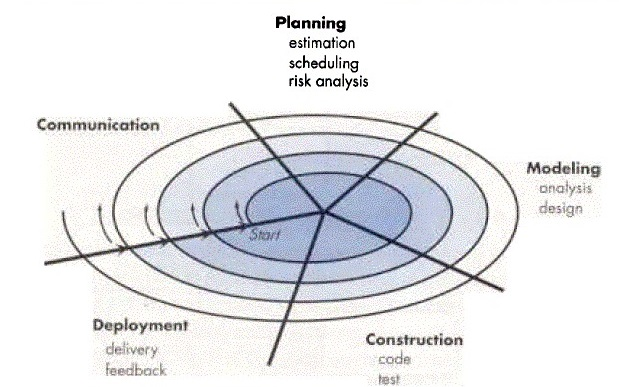
\includegraphics[width=10cm,height=7cm]{gambar/spiral}
	\caption{\textit{Spiral Model}}
	\label{spiral_model}
\end{figure}

Ketika proses pengembangan dimulai, tim rekayasa perangkat lunak bergerak searah jarum mengelilingi spiral tersebut dengan dimulai dari intinya. Lintasan pertama putaran spiral menghasilkan perkembangan dari spesifikasi produk; putaran spiral selanjutnya mungkin dipakai untuk mengembangkan sebuah \textit{prototype} dan secara progresif mengembangkan versi perangkat lunak yang lebih lengkap \cite{Pressman}.

\section{\textit{Unified Modeling Language} (UML)} 

Salah satu tahap dalam pengembangan sistem adalah tahap desain dimana pada tahap ini semua informasi kebutuhan pengguna dan analisis sistem dituangkan kedalam suatu desain perangkat lunak. Mendesain suatu produk perangkat lunak salah satunya dapat menggunakan pemodelan berorientasi objek (OOP). Menurut Haviluddin dalam \textit{Jurnal Informatika Mulawarman Vol 6 No. 1 (2011)}, \textit{Unified Modelling Language} merupakan alat perancangan sistem yang berorientasi pada objek. Secara filosofi UML diilhami oleh konsep yang telah ada yaitu konsep permodelan \textit{Object Oriented} karena konsep ini menganalogikan sistem seperti kehidupan nyata yang didominasi oleh objek dan digambarkan atau dinotasikan dalam simbol-simbol yang cukup spesifik \cite{Haviluddin}.
 
Menurut Ir. M. Farid Azis, M.Kom (2005) berpendapat bahwa UML adalah sekumpulan simbol dan diagram untuk memodelkan perangkat lunak. Desain dalam bentuk simbol dan diagram, kemudian diterjemahkan menjadi kode program. Implementasi kode program dari diagram UML dapat menggunakan bahasa pemrograman apa saja dengan syarat bahasa pemrograman tersebut harus mendukung pemrograman berorientasi objek (OOP) \cite{Azis}. 

Berdasarkan kedua pendapat di atas dapat disimpukan bahwa UML adalah suatu alat yang digunakan untuk memodelkan atau mendesain perangkat lunak dalam bentuk simbol dan diagram dimana sistem dari perangkat lunak tersebut menggunakan pemrograman berorientasi objek (OOP). Jenis UML yang dipergunakan untuk penelitian ini adalah \textit{use case diagram, class diagram}, dan \textit{activity diagram}. 

\subsection{\emph{Use Case Diagram}} 

Menurut Ade Hendini dalam \textit{Jurnal Khatulistiwa Informatika, Vol. IV, No. 2 (2016)}, \textit{Use Case Diagram }merupakan pemodelan untuk kelakuan (\textit{behavior}) sistem informasi yang akan dibuat. \textit{Use case} digunakan untuk mengetahui fungsi apa saja yang ada di dalam sistem informasi dan siapa saja yang berhak menggunakan fungsi-fungsi tersebut \cite{AdeHendini}. Simbol-simbol yang digunakan dalam \textit{Use Case Diagram} yaitu:

%tabel Simbol Use Case Diagram
\begin{table}[H]
	\centering
	\caption{Simbol-simbol \emph{Use Case Diagram} \cite{AdeHendini}}
	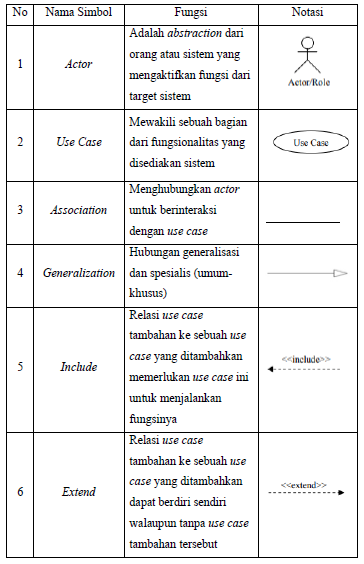
\includegraphics[width=1.0\textwidth]{gambar/simbolusecase}
	\label{tabel_karaktermax2}
\end{table}

\begin{figure}[H]
	\centering
	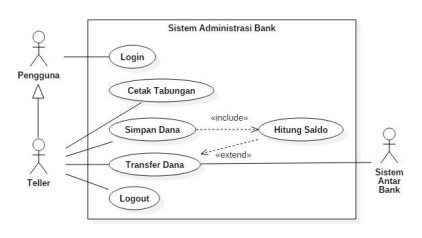
\includegraphics[width=11cm,height=6cm]{gambar/contohusecase}
	\caption{\textit{Contoh \textit{Use Case Diagram}}}
	\label{contoh_usecase}
\end{figure}

\subsection{\emph{Activity Diagram}} 

\emph{Activity Diagram} menggambarkan \textit{workflow} (aliran kerja) atau aktivitas dari sebuah sistem atau proses bisnis \cite{AdeHendini}. Berikut simbol dari activity diagram:

%tabel Simbol Activity Diagram
\begin{table}[H]
	\centering
	\caption{Simbol-simbol \emph{Activity Diagram} \cite{AdeHendini}}
	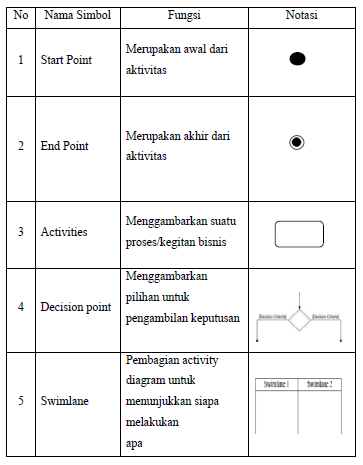
\includegraphics[width=1.0\textwidth]{gambar/simbolactivity}
	\label{tabel_karaktermax2}
\end{table}

\subsection{\emph{Class Diagram}}

\textit{Class diagram} menggambarkan \textit{class} dan hubungan antar-\textit{class} di dalam sisem. 
\textit{Class} digambarkan dengan sebuah kotak dibagi menjadi tiga bagian. Bagian paling atas diisikan nama \textit{class}, 
bagian tengah diisikan variabel yang dimiliki \textit{class} dan bagian bawah diisikan \textit{method} dari \textit{class} \cite{Azis}.

\begin{figure}[H]
	\centering
	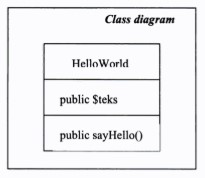
\includegraphics[width=6cm,height=5cm]{gambar/contohclass}
	\caption{\textit{Contoh sederhana \textit{Class Diagram}}}
	\label{contoh_class}
\end{figure}

\textit{Class Diagram} secara khas meliputi: Kelas (\textit{Class}), Relasi Asosiasi/\textit{Associations}, Generalisasi/\textit{Generalization} dan Agregasi/\textit{Aggregation}, atribut (\textit{Attributes}), 
operasi (\textit{operation/method}), dan hubungan antar kelas mempunyai keterangan yang disebut dengan \textit{Multiplicity}
atau \textit{Cardinality}.

\begin{table}[H]
	\centering
	\caption{\emph{Multiplicity Class Diagram}}
	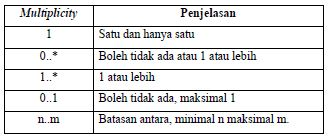
\includegraphics[width=1.0\textwidth]{gambar/multiplicity}
	\label{tabel_karaktermax2}
\end{table}
Berikut simbol-simbol yang terdapat pada\textit{ class diagram} beserta deskripsinya: 
\begin{table}[H]
	\centering
	\caption{Simbol-simbol \emph{Class Diagram} \cite{Rosa}}
	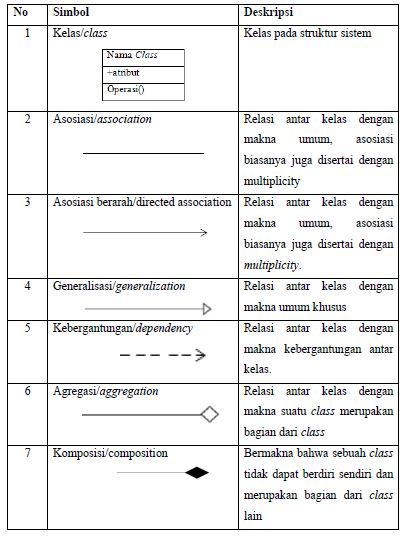
\includegraphics[width=1.0\textwidth]{gambar/simbolclass}
	\label{tabel_karaktermax2}
\end{table}

\section{\emph{Entity Relationship Database}(ERD)}

Komponen utama dari suatu sistem informasi adalah data, data akan diolah menjadi suatu informasi yang digunakan untuk pengambilan keputusan. Salah satu cara dalam memodelkan suatu data ialah dengan menggunakan \textit{Entity Relationship Diagram} (ERD).\textit{ Entity Relationship Diagram} (ERD) adalah sekumpulan cara atau peralatan untuk mendeskripsikan data-data atau objek-objek yang dibuat berdasarkan dan berasal dari dunia nyata yang disebut entitas (\textit{entity}) serta hubungan (\textit{relationship}) antar entitas-entitas tersebut \cite{DoroEdi}. 

Simbol-simbol dalam ERD (\textit{Entity Relationship Diagram}) adalah sebagai berikut \cite{Fridayanthie}.
\begin{enumerate}
	\item Entitas: suatu yang nyata atau abstrak yang mempunyai karakteristik dimana kita akan menyimpan data.
	\item Atribut: ciri umum semua atau sebagian besar instansi pada entitas tertentu.
	\item Relasi: hubungan alamiah yang terjadi antara satu atau lebih entitas. Jenis relasi yang ada pada ERD, yaitu one-to-one, one-to-many, dan many-to-many.
	
\end{enumerate}



\section{\emph{Model View Controller} (MVC)}

MVC merupakan arsitektur yang membagi aplikasi menjadi tiga bagian secara konsep yang terpisah yaitu \textit{Model}, \textit{View}, dan \textit{Controller}, masing-masing dapat dikembangkan secara terpisah antara satu dengan yang lainnya, sehingga perubahan pada satu bagian memiliki dampak minimal pada bagian lain. Bagian model digunakan untuk mendefinisikan suatu cara dimana data dapat diakses, bagian view menghasilkan keluaran jika diberikan data, dan bagian controller menerima perintah dan mengatur aplikasi untuk tugas dan tampilan yang sesuai \cite{AriefHidayat}. 

Untuk lebih jelasnya berikut tiga komponen yang membangun MVC \cite{Wellem} :
\begin{enumerate}
	\item Model, digunakan untuk mengelola informasi atau data dan merepresentasikannya kepada pengguna. Pada umumnya, \textit{Model} berisi fungsi-fungsi yang berhubungan dengan \textit{database}, seperti pengambilan data, \textit{update} data, \textit{insert} data, \textit{delete} data, dan lain sebagainya.
	\item \textit{View}, merupakan informasi yang direpresentasikan kepada pengguna. \textit{View} biasanya berupa halaman web, dimana pengguna dapat melihat informasi yang ditampilkan.
	\item \textit{Controller}, memberikan pelayanan yang menjembatani \textit{Model} dan \textit{View}. \textit{Controller} berisi fungsi-fungsi yang dapat membantu menjembatani \textit{Model} dan \textit{View}. Request datang dan di-\textit{response} melalui \textit{Controller}, kemudian \textit{Controller} berkomunikasi serta melakukan kontrol terhadap \textit{View} dan \textit{Model}.
\end{enumerate}

\begin{figure}[H]
	\centering
	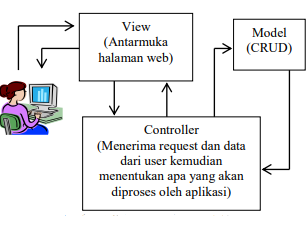
\includegraphics[width=7cm,height=5cm]{gambar/alurmvc}
	\caption{Alur Kerja MVC}
	\label{alurmvc}
\end{figure}

MVC dimulai pada saat pengguna memulai mengakses aplikasi. Awalnya pengguna akan menjalankan operasi pada bagian \textit{View}. Proses ini dapat berupa proses\textit{ Login}, Pendaftaran ataupun proses lainnya. Kemudian perintah akan direspon oleh bagian \textit{Controller}. Bagian\textit{ Controller} akan menentukan apakah permintaan dari pengguna akan diproses atau tidak, ketika diproses maka permintaan akan diarahkan ke bagian\textit{ Model}. Setelah permintaan dari pengguna dapat dipenuhi oleh \textit{model} maka informasi akan dikirimkan kembali ke bagian \textit{controller} lalu diberikan ke bagian \textit{view} sehingga pengguna dapat memperoleh informasi sesuai yang diinginkan \cite{Martono}.

\section{Basis Data} 

Basis data terdiri dari dua kata, yaitu basis dan data. Basis dapat diartikan sebagai markas, gudang, dan tempat berkumpul. Sedangkan data adalah fakta yang mewakili suatu objek seperti manusia, barang hewan, peristiwa dan sebagainya, yang direkam dalam bentuk angka, huruf, simbol, teks, gambar, bunyi atau kombinasinya. Menurut Robi Yanto, M.Kom basis data dapat didefinisikan sebagai himpunan kelompok data yang saling berhubungan yang diorganisasi sedemikian rupa agar dapat dimanfaatkan kembali dengan cepat dan mudah \cite{Robi}. 

Sedangkan menurut Edhy Sutanta basis data dapat dipahami sebagai suatu kumpulan data terhubung (\textit{interrelatet data}) yang disimpan secara bersama-sama pada suatu media, data disimpan dengan cara-cara tertentu sehingga mudah untuk digunakan atau ditampilkan kembali; data dapat digunakan oleh satu atau lebih program-program aplikasi secara optimal; data disimpan sedemikian rupa sehingga proses penambahan, pengambilan, dan modifikasi data dapat dilakukan dengan mudah dan terkontrol \cite{Edhy}. 

Berdasarkan dari kedua pendapat tersebut, basis data dapat dikatakan merupakan sekumpulan kelompok data yang saling terhubung satu sama lain, disimpan dan diatur sedemikian rupa pada suatu media agar data dapat diambil dan dikelola dengan mudah. 

Sistem adalah sekumpulan komponen-komponen yang saling berhubungan dan secara bersama-sama bertujuan untuk memenuhi suatu pekerjaan tertentu. Komponen penting dalam sistem basis data adalah \cite{Robi}:

\begin{enumerate}
	\item Data
	
	Merupakan informasi yang disimpan dalam suatu struktur tertentu yang terintegrasi
	\item \textit{Hardware}
	
	Merupakan perangkat keras berupa komputer dengan media penyimpanan data karena pada umumnya basis data memiliki ukuran yang besar
	\item Sistem Operasi
	
	Program yang mengaktifkan dan memfungsikan sistem komputer, mengendalikan seluruh sumber daya dalam komputer, dan melakukan operasi dasar dalam komputer meliputi input, proses, dan output. 
	\item Basis Data
	
	Sebagai inti dari sistem basis data. Basis data menyimpan data serta struktur sistem basis data baik untuk entitas maupun objek-objek secara detail.
	\item \textit{Database Management System}
	
	Merupakan perangkat lunak yang digunakan untuk melakukan pengelolaan basis data sebagai contoh \textit{Microsoft access, Sql Server, Mysql}, dan \textit{Oracle}. 
	\item \textit{User}
	
	Merupakan pengguna yang menggunakan data yang tersimpan dan terkelola. \textit{User} dapat berupa seseorang yang mengelola basis data yang disebut database administrator (DBA), bisa juga disebut \textit{end user}. 
\end{enumerate}

Basis data dapat digolongkan berdasarkan beberapa kriteria, salah satunya ialah berdasarkan seberapa sering basis data mengalami perubahan dikenal dua penkategorian yaitu \cite{Sulianta} :

\begin{enumerate}
	\item Tabel/data master adalah tabel yang datanya cenderung jarang berubah dan tidak memiliki ketergantungan dengan tabel lain.
	\item Tabel/data transaksi adalah tabel yang datanya sering berubah dan membutuhkan data master untuk membangun komponennya 
\end{enumerate}

		
% Baris ini digunakan untuk membantu dalam melakukan sitasi
% Karena diapit dengan comment, maka baris ini akan diabaikan
% oleh compiler LaTeX.
\begin{comment}
bibliography{daftar-pustaka}
\end{comment}
